\subsubsection{\stid{3.13} CLOVER Sub-project: heFFTe}\label{subsubsect:fftecp}


\paragraph{Overview}

The {\it Highly Efficient FFTs for Exascale} ({\bf heFFTe}) project provides sustainable 
high-performance multidimensional Fast Fourier Transforms (FFTs) for Exascale 
platforms~\cite{thasd19,heffte-iccs20}.
HeFFTe leverages established but {\it ad hoc} 
software tools that have traditionally been part of application 
codes, but not extracted as independent, supported libraries. 
%
The main objective of the heFFTe project is to:
%\begin{itemize}
%\item
1)~ 
      Collect existing FFT capabilities from ECP 
      application teams;
%\item 
2)~
      Assess gaps, extend, and make available various FFT
      capabilities as a sustainable math library;
%\item 
3)~      
      Explore opportunities to build multidimensional FFTs
      while leveraging on-node concurrency from 
      batched FFT formulations;
%\item
4)~
      Focus on capabilities for Exascale platforms.
%\end{itemize}

FFTs are used in many applications including molecular dynamics, 
spectrum estimation, fast convolution and correlation, signal 
modulation and many wireless multimedia applications. The 
distributed 3D FFT is one of the most important routines used 
in molecular dynamics (MD) computations, and its performance can 
affect MD scalability. The performance of the first 
principles calculations strongly depends on the performance of the 
FFT solver that performs many FFTs of size $\approx 10^7$ points in 
a calculation that we call batched FFT. Moreover, Poisson PDE-type 
equations arising from many engineering areas, such as plasma
simulation and density fields, need to solve FFTs of size larger than $10^9$. 
%
More than a dozen ECP applications use FFT in their codes.
ECP applications that require FFT-based solvers suffer from the lack of 
fast and scalable 3D FFT routines for distributed-heterogeneous parallel 
systems as the ones projected for the upcoming exascale computing systems. 
To address these needs, heFFTe functionalities are first delivered 
to CoPA projects using LAMMPS (molecular dynamics) and HACC (Hardware Accelerated
Cosmology Code).

The heFFTe software stack is illustrated in the left-hand side of Figure~\ref{fig:fft-ecp-pipeline}, 
while the main components of the heFFTe framework are illustrated in the right-hand side of
Figure~\ref{fig:fft-ecp-pipeline}. 
% The first and last step address the need 
% for a flexible FFT API to take application-specific input and output (bricks/pencils), 
% including arbitrary initial decompositions. 
% Currently, heFFTe provides efficient
% GPU support for all communication primitives and features in FFTMPI and SWFFT.
 
\begin{figure}[htb]
    \centering
    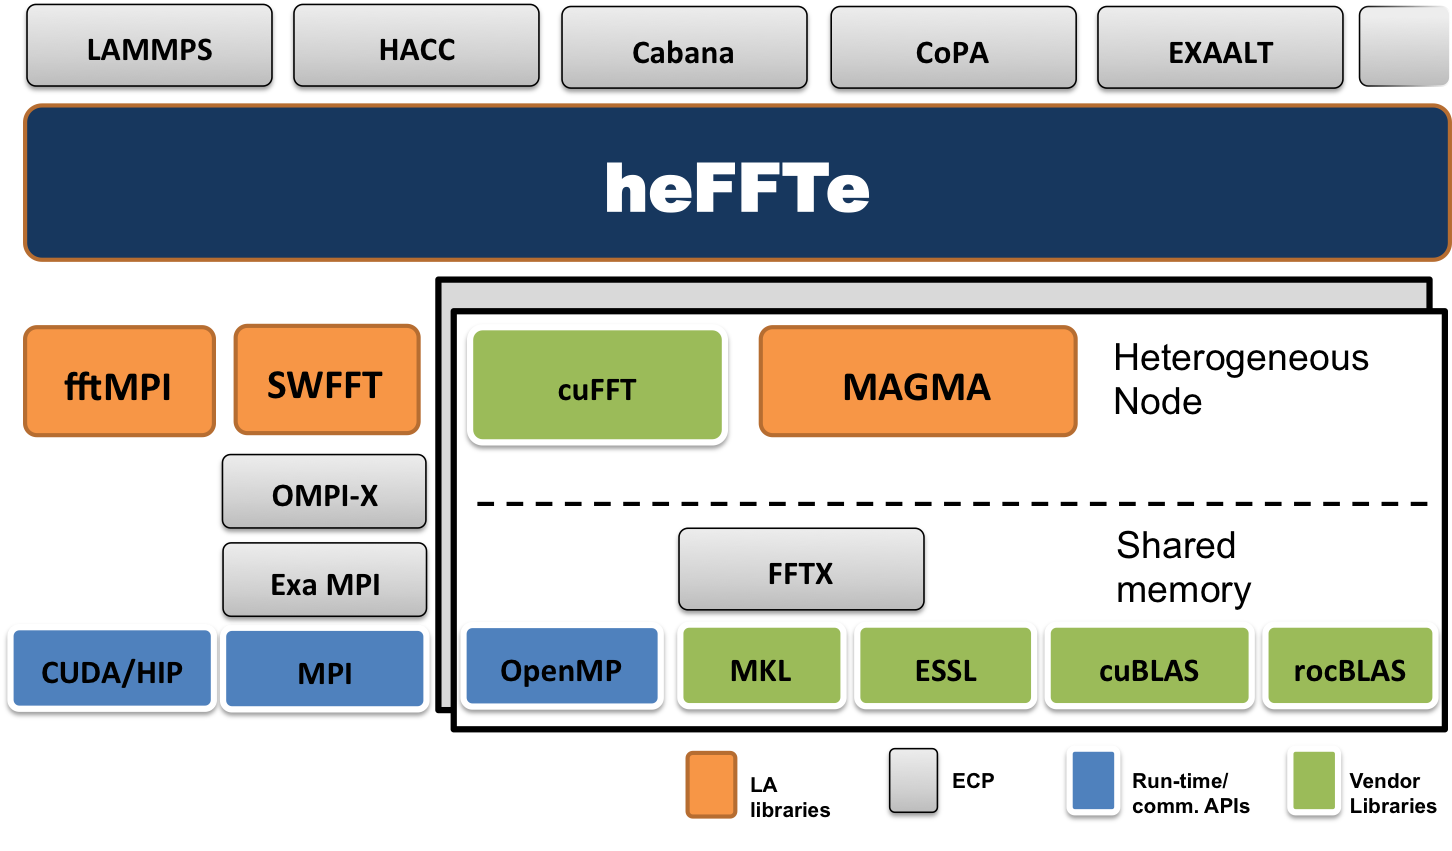
\includegraphics[width=0.42\textwidth]{projects/2.3.3-MathLibs/2.3.3.13-CLOVER/heffte}~~
    \raisebox{.4\height}{\includegraphics[width=0.56\textwidth]{projects/2.3.3-MathLibs/2.3.3.13-CLOVER/ffttransormations}}
    \caption{\label{fig:fft-ecp-pipeline}
    {\bf Left}: the heFFTe software stack. {\bf Right}: 3D FFT computational pipeline in heFFTe with:~
      1) Flexible API for application-specific input and output,
         including bricks/pencils/etc.;~
      2) Efficient packing/unpacking and MPI communication
         routines;~
      3) Efficient 1D/2D/3D FFTs on the node.}
\end{figure}

\paragraph{Key  Challenges}
\begin{enumerate}
\item
\textbf{Communication costs:}
%Today's machines have very complex memory hierarchies and thus data movement, 
%data layout translation, and communication should be the main focus of any 
%distributed FFT library that aims to improve the performance of any ECP 
%application that relies on FFT. 
Communication costs are main bottleneck 
on current systems; this includes low node bandwidth (relative to 
high compute capabilities) and sub-optimal accelerator-aware MPI 
communications that can lead to some stong scalability issues~\cite{heffte-pact21}.

\item
\textbf{Application specifics:}
ECP applications that require FFT-based solvers suffer from the lack of fast 
and scalable FFTs for distributed-heterogeneous parallel systems 
as the ones projected for the upcoming exascale computing systems. Also, ECP 
applications need different application-specific versions of FFTs,
and dictate parallelism and data distributions (where is the data, how is 
distributed, what is the parallelism, etc.). This requires application
knowledge and API designs with a suitable modular high-performance 
implementation that is flexible and easy to use and integrate in ECP applications.

\item
\textbf{Performance portability:}
Performance portability across different architectures is always a challenge.
This is further exacerbated due to the many application and 
hardware-specific FFT versions needed.
\end{enumerate}

\paragraph{Solution Strategy}

\begin{enumerate}
\item
\textbf{Communications and GPU optimizations:}
FFTs are communication bound and a main focus in heFFTe is on algorithmic
design to minimize communication and efficient GPU 
implementations~\cite{sc19,eurompi19,heffte-pact21,hpec21}.
Other strategies include the use of mixed-precision calculations~\cite{Haidar2018,tcfft18}
and data compression for reduced communications (including lossy, e.g., using ZFP 
compression)~\cite{Anztetal2020}.
\item
\textbf{Evolving design:}
heFFTe is designed to support the fftMPI and SWFFT functionalities,
which are already integrated in ECP applications. Thus, heFFTe benefits
directly these applications and provides integrated solutions. 
More functionalities and application-specific optimizations will be added 
through heFFTe backends to support various ECP applications. 
\item
\textbf{Autotuning:}
Performance portability will be addressed through use of standards (like 1D FFTs 
from vendors), portable linear algebra (LA) using MAGMA~\cite{Tomov_2010_pcsa}, 
and parameterized versions that will be tuned across architectures. We have extensive 
expertise and well proven track record in the development and use of autotuning techniques 
for important LA kernels~\cite{Nath2010,Kurzak2012gemmfermi}. 
\end{enumerate}

\paragraph{Recent Progress}
The heFFTe team completed two main milestones involving software releases adding 
numerous stability, performance, and scalability enhancements, as well as new 
functionalities~\cite{heffte-pact21}. 
HeFFTe 2.1 was released in April 2021, and heFFTe 2.2 was released in October 
2021. HeFFTe 2.1 added support for multidimensional FFTs and optimizations for real data.
This included the development of R2C and C2R FFTs and their integration in heFFTe and 
specific optimizations in ECP applications. Support and optimizations was extended for AMD 
GPUs, dependence on MAGMA was added, as well as spack installation, and integration of heFFTe in xSDK.
HeFFTe was also integrated in CoPA projects and ExaAM/Meumapps with new application-specific 
optimizations, tuning, and added Intel GPU support. 
HeFFTe 2.2 concentrated on adding support and optimization of the HIP and Intel GPU backends to 
heFFTe. HeFFTe's functional and performance portability on these architectures and
multicore CPUs was established~\cite{hpec21}, as well as ease of integration in the ECP applications 
using heFFTe. 
Multidimensional FFTs for 
fast discrete convolution, cosine (DCT), and sine (DST) transforms were also added with support 
for Nvidia, AMD, 
and Intel GPUs. HeFFTe has demonstrate very good strong scalability and performance that is 
close to 90\% of the roofline peak on the newly added in heFFTe v2.2 R2C, C2R, convolution,
DCS and DST transformations~\cite{heffte-pact21,heffte-iccs20} (see Figure~\ref{fig:fft-ecp-progress}). 
An FFT benchmark for a number of FFT libraries, including a design study and evaluation of FFT 
codes used in the ECP applications, was also developed~\cite{fftbenchmark}.

\begin{figure}[htb]
   \centering
%   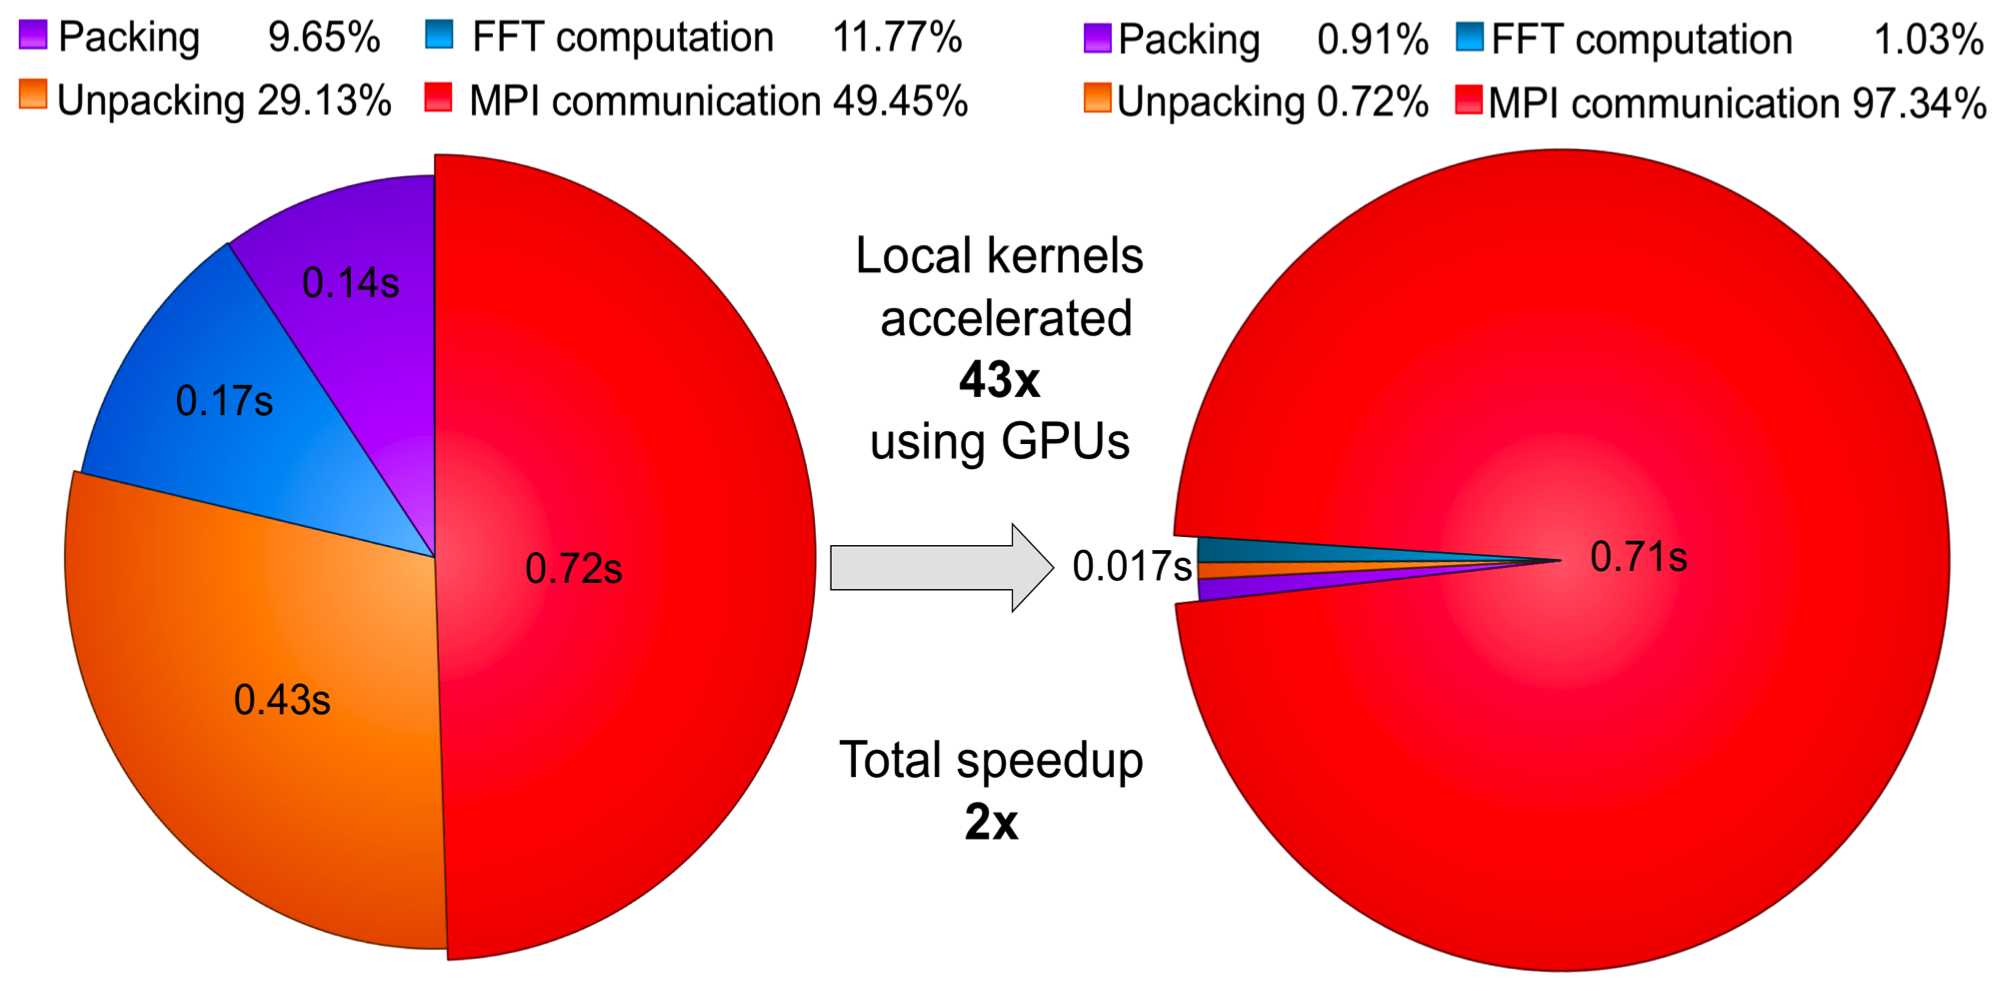
\includegraphics[width=0.55\textwidth]{projects/2.3.3-MathLibs/2.3.3.13-CLOVER/heFFTeAcceleration}~~~
   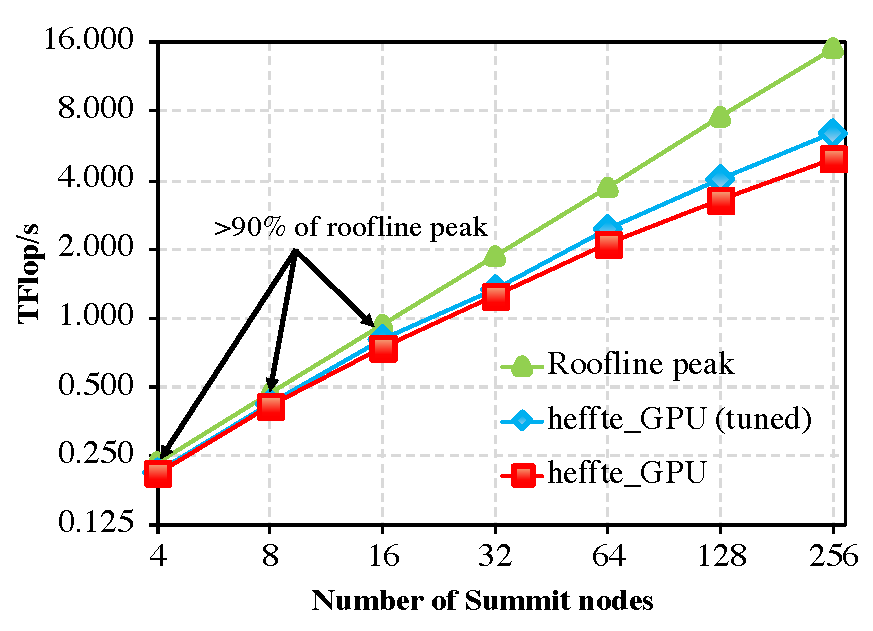
\includegraphics[width=0.32\textwidth]{projects/2.3.3-MathLibs/2.3.3.13-CLOVER/heFFTeStrongScalability}
   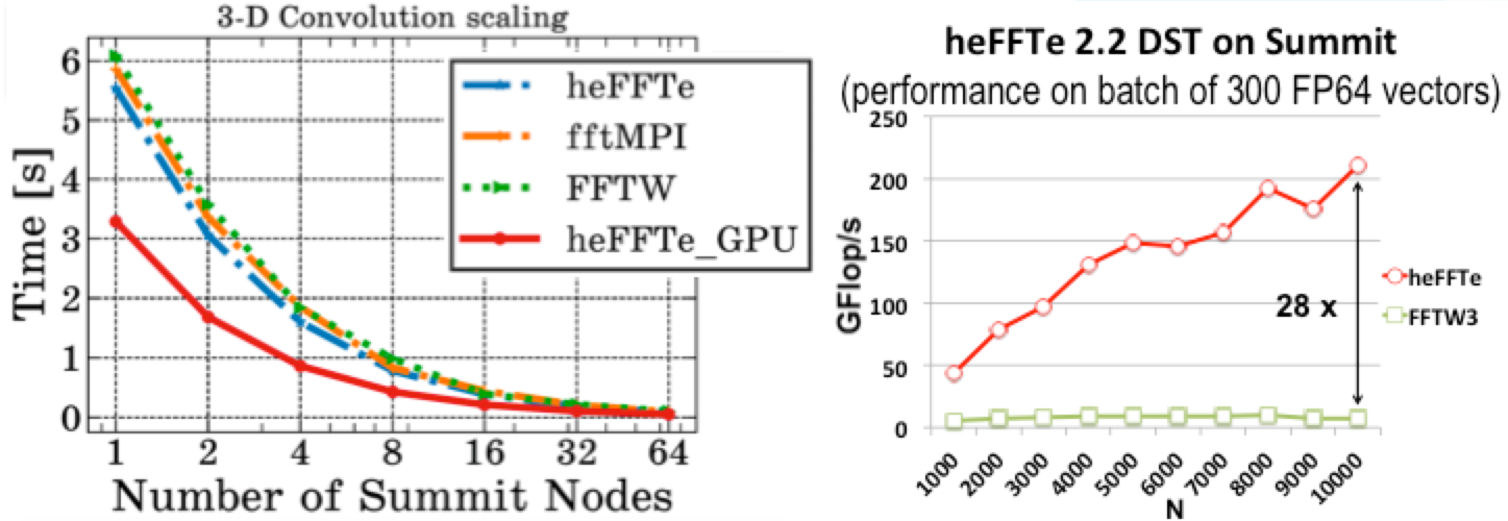
\includegraphics[width=0.65\textwidth]{projects/2.3.3-MathLibs/2.3.3.13-CLOVER/heffte_conv_dst}
    \caption{\label{fig:fft-ecp-progress}
    %{\bf Left}: heFFTe acceleration of $1024^3$ FFT on 4 Summit nodes.
    %            Note: nodal computations are accelerated $43\times$. 
    {\bf Left}: heFFTe strong scalability on $1024^3$ 
                FFT on up to 256 nodes ($\times 6$ V100 GPUs;
                double complex arithmetic; starting and ending with bricks; 
                performance assumes $5 N^3 log_2 N^3$ flops).
    {\bf Middle}: Convolution of $512^3$ multidimensional arrays in double complex arithmetic.
    {\bf Right}: Performance of the Discrete Sine Transformation (DST) in heFFTe 2.2.
    }
\end{figure}


\paragraph{Next Steps}
Next steps of work are adding multidimensional batched FFTs and optimizations.
This will include support for AMD, Nvidia, and Intel GPUs.
Further integration and use will be added to CoPA applications and the ExaAM project.
Autotuning framework that hides backend selection and other parameters from users
will be added, as well as improved GPU-aware MPI Alltoallv routines, mixed-precision, 
and approximate FFTs. Existing FFT libraries will be evaluated through the FFT 
benchmark~\cite{fftbenchmark}.



